\documentclass[14pt]{extarticle}

\usepackage{fontspec}
\setmainfont{Times New Roman}

% размер полей
\usepackage{geometry}
\geometry{a4paper, top=2cm, bottom=2cm, right=1.5cm, left=3cm}

 %debugging
%\usepackage{showframe}

% полуторный интервал
\usepackage{setspace}
\onehalfspacing

% абзацный отступ
\setlength{\parindent}{1.25cm}

% выравнивание текста по ширине
\sloppy

% списки
\usepackage{calc} % арифметические операции с величинами
\usepackage{enumitem}
\setlist{
    nosep,
    leftmargin=0pt,
    itemindent=\parindent + \labelwidth - \labelsep,
}

% подписи к рисункам и таблицам
\usepackage{caption}
\renewcommand{\figurename}{Рисунок}
\renewcommand{\tablename}{Таблица}
\DeclareCaptionFormat{custom}
{
    \textit{#1#2#3}
}
\DeclareCaptionLabelSeparator{custom}{. }
\captionsetup{
    % хз какой это размер - 12 или нет, но выглядит меньше 14
    font=small,
    format=custom,
    labelsep=custom,
}

% картинки
\usepackage{graphicx}

% колонтитулы
\usepackage{fancyhdr}

% картинки и таблицы находятся именно в том месте текста где помещены (атрибут H)
\usepackage{float}

% таблицы
\usepackage{tabularray}

\graphicspath{ {3.2.2/models/} }
\begin{document}
\pagestyle{fancy}
\fancyhead{}
% disable header
\renewcommand{\headrulewidth}{0pt}
\fancyfoot[L]{Дубровских гр 221-361}
\fancyfoot[C]{ЛР 3.2.2}
\fancyfoot[R]{Продажа автотранспорта}
\singlespacing

\newpage
\begin{center}
    Министерство науки и высшего образования Российской Федерации
    Федеральное государственное автономное образовательное учреждение

    высшего образования

    \guillemotleft МОСКОВСКИЙ ПОЛИТЕХНИЧЕСКИЙ УНИВЕРСИТЕТ\guillemotright

    (МОСКОВСКИЙ ПОЛИТЕХ)
\end{center}
\noindent
\bigbreak
\bigbreak
\bigbreak
\bigbreak
\begin{center}
    ЛАБОРАТОРНАЯ РАБОТА 5.2.1

    По курсу Проектирования пользовательских интерфейсов в веб

    \textbf{Проектирование композиции и визуальной иерархии в макете веб-страниц и мобильного устройства}
    \bigbreak
    \bigbreak
    \bigbreak
    \bigbreak
    ТЕМА

    \guillemotleft\textbf{САЙТ ДЛЯ ПРОДАЖИ И ПОИСКА АВТОМОБИЛЕЙ}\guillemotright
\end{center}
\noindent
\bigbreak
\bigbreak
\bigbreak
\bigbreak
\bigbreak
\bigbreak
\bigbreak
\bigbreak
\bigbreak
\bigbreak
\hfill Выполнил

\hfill Дубровских Никита Евгеньевич

\hfill Группа 221-361
\bigbreak
\bigbreak
\bigbreak
\hfill Проверил

\hfill Натур ВВ
\vfill
\begin{center}
    Москва, 2024
\end{center}
\newpage
\onehalfspacing


\begin{center}
    \textbf{Лабораторная работа 3.2.2}

    \textbf{Анализ структуры и основных блоков и элементов страниц веб-сайтов}
\end{center}

\textbf{Цель работы:} познакомиться со структурными элементами интерфейса и приемами их расположения на примере сайтов и приложений
\bigskip

\textbf{Задачи:}

\begin{enumerate}
    \item Изучить структуру и найти основные блоки и элементы страниц веб-сайтов.
    \item Изучить паттерны сканирования экрана (айтрекинг) пользователями, "Тепловые карты" сайтов, карты скроллинга и кликов мыши, диаграмму Гутенберга и найти их использование в интерфейсах  сайтов 
    \item Изучить приемы композиции на примере расположения элементов и блоков интерфейса сайтов.

\end{enumerate}
\bigskip

\textbf{Основные термины}

\begin{itemize}
    \item Структурные элементы интерфейса - основные компоненты, из которых состоит веб-сайт или приложение.
    \item Блоки и элементы страниц - различные части веб-страницы, такие как заголовки, подвал, навигация и т.д.
    \item Тепловые карты - визуальные представления, показывающие, где пользователи кликают на сайте.
    \item Карта скроллинга - анализ того, как далеко пользователи прокручивают страницу.
    \item Диаграмма Гутенберга - схема, показывающая, как пользователи воспринимают информацию на странице.
    \item Композиция - приемы расположения элементов и блоков интерфейса для создания визуально привлекательного дизайна.
    \item Модальное окно - элемент интерфейса, который требует взаимодействия пользователя перед тем, как он сможет продолжить.
    \item Чекбокс - элемент управления, позволяющий пользователю выбрать один или несколько вариантов.
    \item Фавикон - маленькая иконка, представляющая сайт в браузере.
    \item Футер (подвал) - нижняя часть веб-страницы, содержащая дополнительную информацию.
    \item Пагинация - система навигации, позволяющая пользователям перемещаться между страницами.
    \item Хлебные крошки - навигационный элемент, показывающий путь к текущей странице.
    \item Кнопка CTA (Call to Action) - элемент, призывающий пользователя к действию.
    \item Сниппет - краткое описание содержимого страницы, отображаемое в результатах поиска.
    \item Рейтинг бар - визуальный индикатор оценки или рейтинга.
    \item Слайдер - элемент интерфейса, позволяющий пользователю прокручивать изображения или контент.
    \item Галерея - коллекция изображений или медиа-контента, представленных в одном месте.
\end{itemize}
\bigskip

\textbf{Структура сайта}
\bigskip

\noindent
\begin{minipage}{\linewidth}
    \fbox{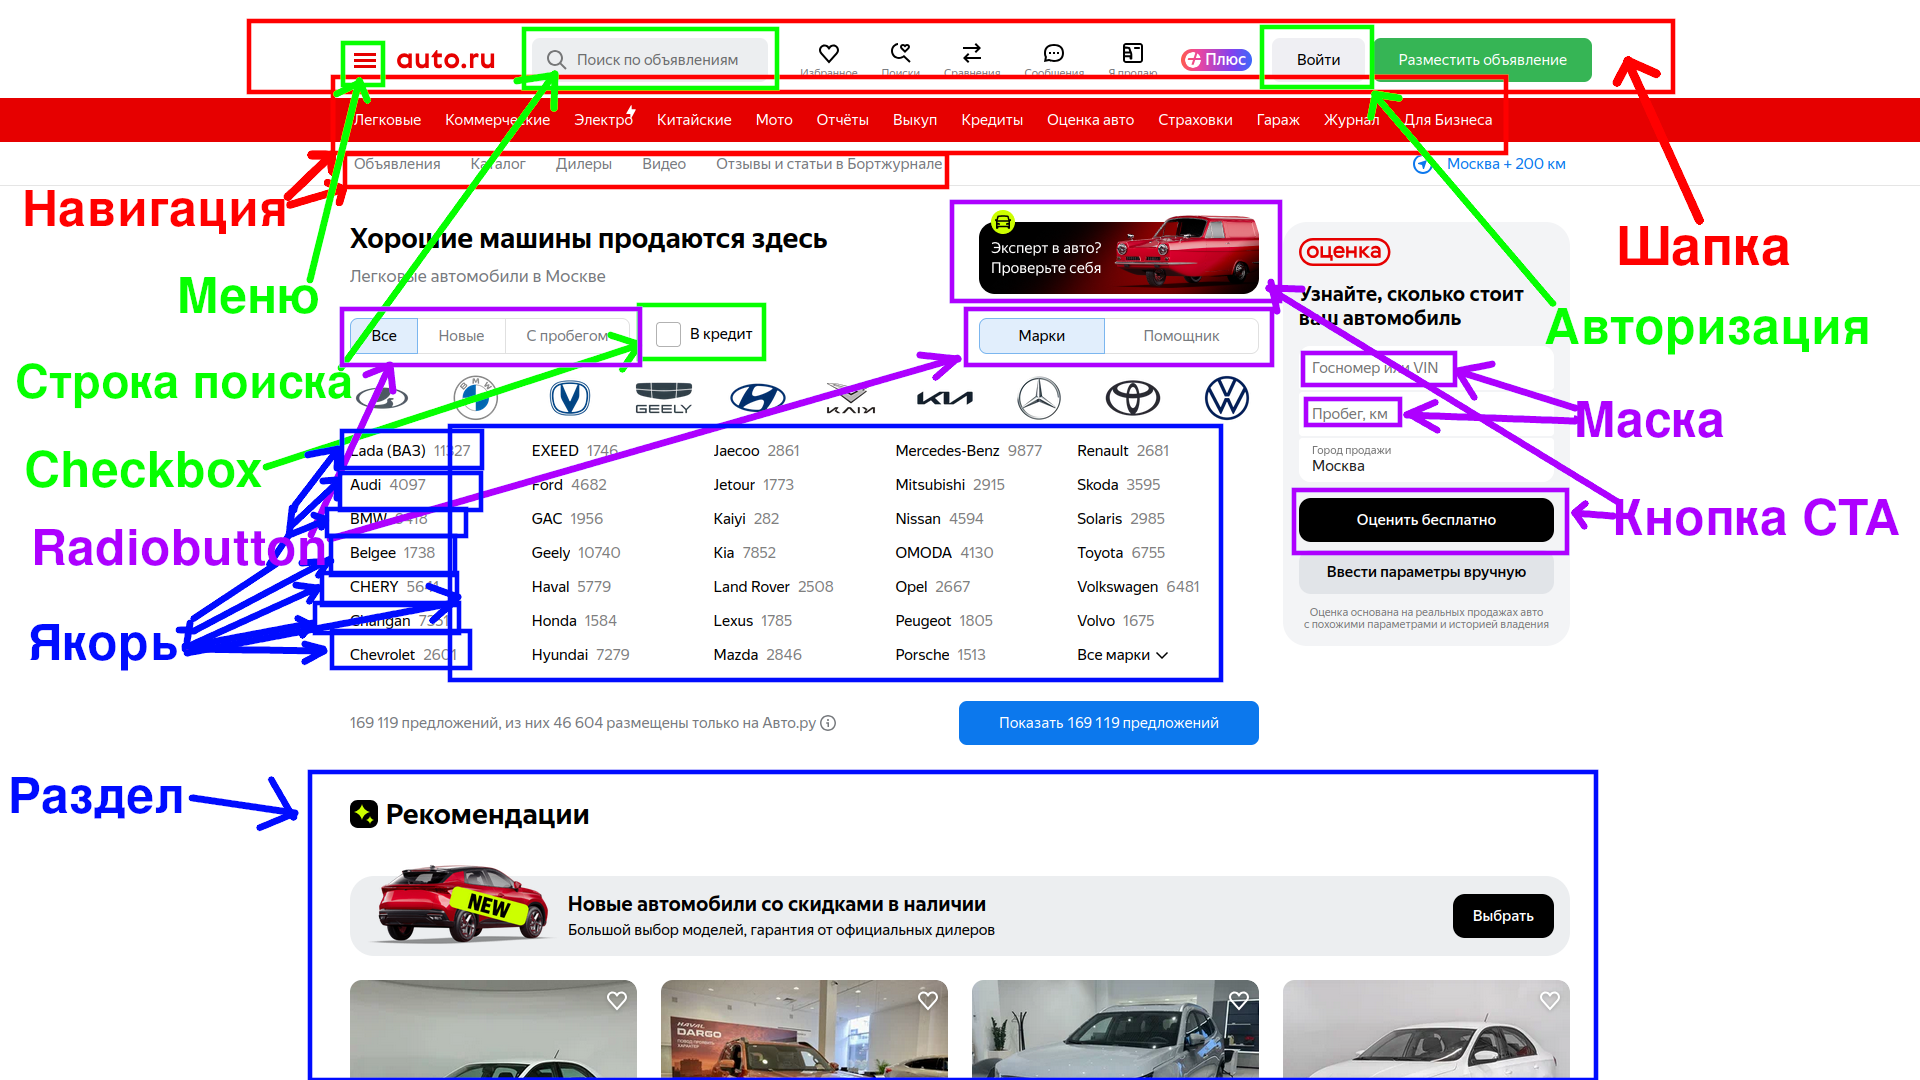
\includegraphics[width=\linewidth]{auto_ru_main_page}}
    \captionof{figure}{Структура сайта auto.ru}
\end{minipage}
\bigskip

\noindent
\begin{minipage}{\linewidth}
    \fbox{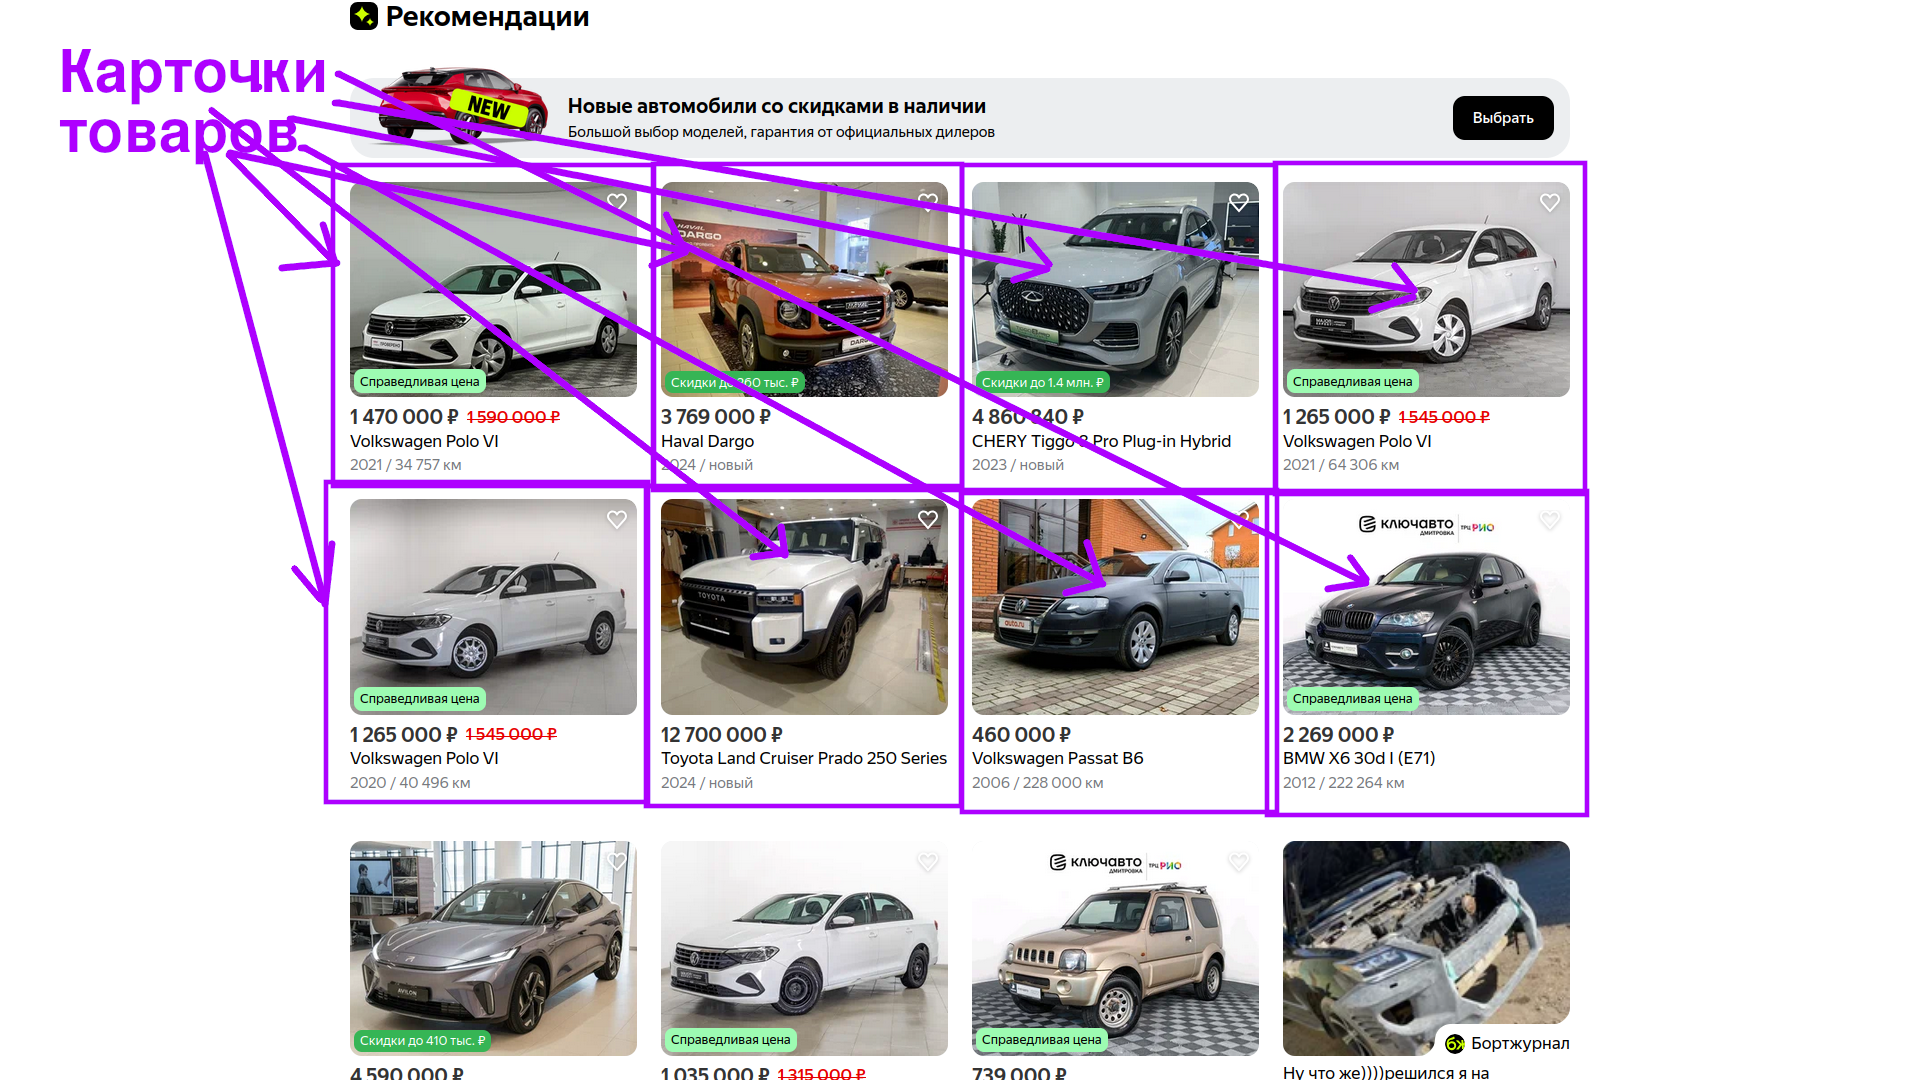
\includegraphics[width=\linewidth]{auto_ru_cards}}
    \captionof{figure}{Структура сайта auto.ru}
\end{minipage}
\bigskip

\noindent
\begin{minipage}{\linewidth}
    \fbox{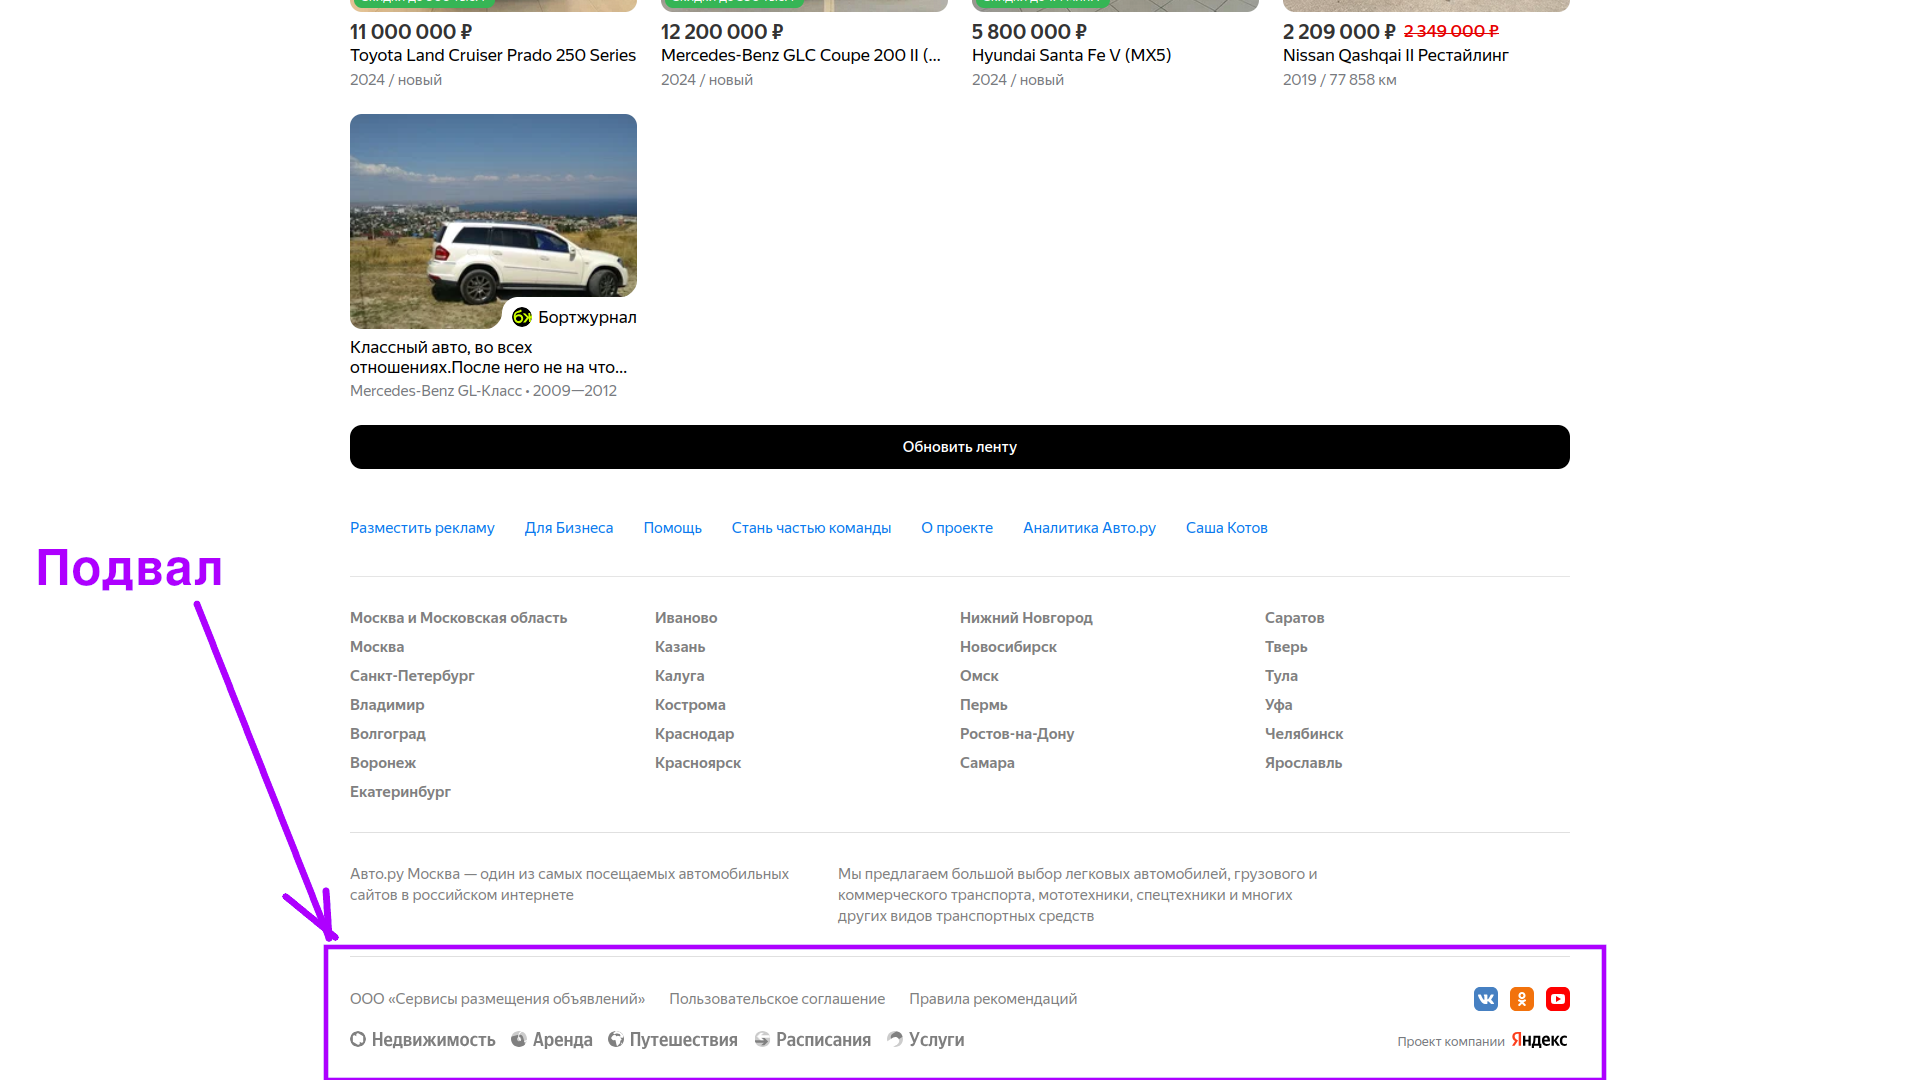
\includegraphics[width=\linewidth]{auto_ru_footer}}
    \captionof{figure}{Структура сайта auto.ru}
\end{minipage}
\bigskip

\textbf{Контрольные вопросы и ответы}

\begin{enumerate}
    \item Какие структурные элементы страниц Вам известны?

    Заголовок (Header), подвал (Footer), навигационное меню, боковые панели (Sidebar), контентные блоки, карточки товаров, формы, кнопки, изображения, слайдеры, хлебные крошки и пагинацию.
    \item Чем отличается внешняя и внутренняя структура Веб-страниц?

    Внешняя структура веб-страницы относится к тому, как страница выглядит для пользователя, включая визуальные элементы и их расположение. Внутренняя структура касается организации кода и данных, таких как HTML, CSS и JavaScript, которые определяют функциональность и поведение страницы.
    \item Какие структурные используются для навигации страниц? Виды навигации.

    Для навигации страниц используются элементы, такие как навигационное меню, хлебные крошки, пагинация, ссылки на другие страницы и кнопки "Назад" и "Вперед". Виды навигации включают горизонтальную, вертикальную, фиксированную, выпадающую и контекстную навигацию.
    \item Для чего предназначены структурные элементы Модальное окно, Чекбокс, Маска?

    Модальное окно предназначено для отображения важной информации или запроса действий от пользователя, не позволяя взаимодействовать с остальной частью страницы. Чекбокс позволяет пользователю выбрать один или несколько вариантов из предложенного списка. Маска используется для ограничения ввода данных в определенном формате (например, телефонные номера).
    \item Для чего предназначены структурные элементы Фавикон, Футер, Подвал, Сниппет?

    Фавикон — это иконка, представляющая сайт в браузере и закладках. Футер (подвал) содержит дополнительную информацию, такую как контактные данные, ссылки на политику конфиденциальности и условия использования. Сниппет — это краткое описание содержимого страницы, отображаемое в результатах поиска, помогающее пользователям понять, о чем страница.
    \item Для чего предназначены структурные элементы Пагинация, Хлебные крошки, Превью, кнопка СТА?

    Пагинация позволяет пользователям перемещаться между страницами контента. Хлебные крошки показывают путь к текущей странице, облегчая навигацию. Превью предоставляет краткий обзор содержимого, например, изображение или текст. Кнопка CTA (Call to Action) призывает пользователя к конкретному действию, например, "Купить сейчас" или "Подписаться".
    \item Что такое паттерны сканирования экрана (айтрекинг) пользователями, "Тепловые карты" сайтов?

    Паттерны сканирования экрана (айтрекинг) описывают, как пользователи просматривают и воспринимают информацию на странице. "Тепловые карты" визуализируют, где пользователи кликают, прокручивают или задерживают взгляд, показывая наиболее активные области на сайте.
    \item Какие примы композиции могут быть использованы в интерфейсе сайтов (мобильных приложений)?

    Приемы композиции включают использование сеток для организации элементов, контраст для выделения важных частей, баланс между текстом и изображениями, иерархию для упорядочивания информации, а также использование белого пространства для улучшения читаемости и восприятия.
\end{enumerate}

\end{document}
